\documentclass[11pt,letterpaper]{article}
\usepackage[margin=1in]{geometry}
\usepackage{graphicx}
\usepackage{booktabs}
\usepackage{amsmath,amssymb}
\usepackage{hyperref}
\usepackage{xcolor}
\usepackage{caption}
\usepackage{subcaption}
\usepackage{float}
\usepackage{enumitem}
\usepackage{titlesec}
\usepackage{parskip}
\usepackage{microtype}
\usepackage{cite}
\usepackage{listings}

\hypersetup{colorlinks=true,linkcolor=blue!60!black,citecolor=blue!60!black,urlcolor=blue!60!black}
\captionsetup{font=small,labelfont=bf}
\setlength{\parskip}{6pt}

\title{\textbf{Scaling Laws for Transformer Language Models\\Trained on SVG Code}\\[4pt]
\large CS-GY 6923 Optional Project\\
New York University Tandon School of Engineering}
\author{[Your Name Here]}
\date{May 2026}

\begin{document}
\maketitle
\tableofcontents
\newpage

% ─────────────────────────────────────────────────────────────────────────────
\section{Introduction}
% ─────────────────────────────────────────────────────────────────────────────

Neural scaling laws—the observation that model performance improves predictably with parameter
count and data quantity—have reshaped how large language models (LLMs) are developed
\cite{kaplan2020scaling,hoffmann2022chinchilla}. However, these laws were derived primarily on
natural-language text. A natural question is: \emph{do the same power-law relationships hold in
structured, non-linguistic domains?}

Scalable Vector Graphics (SVG) is an ideal testbed for this question. Unlike natural language,
SVG is governed by strict syntactic rules (valid XML), a hierarchical coordinate system, and
a closed vocabulary of element types and attributes. Crucially, SVG outputs can be
\emph{instantly rendered} in any browser, enabling both quantitative (perplexity, XML validity)
and qualitative (visual coherence) evaluation—a rare luxury in language modeling research.

\textbf{Our approach.}~We train a family of five decoder-only Transformer models (1M–88M
non-embedding parameters) on a corpus of $\sim$128M tokens of simplified SVG icons and emoji.
We:
\begin{enumerate}[nosep]
  \item Build a full preprocessing pipeline—SVG cleaning, BPE tokenization, and train/val/test splits.
  \item Empirically derive power-law scaling curves $L = a \cdot N^{-\alpha} + c$ under
        standard parameterization (SP).
  \item Investigate Maximal Update Parameterization ($\mu$P) as a principled alternative for
        hyperparameter transfer across widths.
  \item Generate and evaluate SVG samples from the best-trained model.
\end{enumerate}

This work contributes empirical evidence for scaling laws in a structured code domain, and
investigates whether $\mu$P's zero-shot learning-rate transfer benefits transfer to non-NLP
domains.

% ─────────────────────────────────────────────────────────────────────────────
\section{Data}
% ─────────────────────────────────────────────────────────────────────────────

\subsection{Dataset Description}

Our primary dataset is \texttt{starvector/svg-icons-simple} \cite{rodriguez2023starvector},
containing $\sim$89,370 simplified SVG icons (153 MB). We supplement this with
\texttt{starvector/svg-emoji-simple} (8,421 emoji SVGs) and a 50,000-example subsample of
\texttt{starvector/svg-fonts-simple} to reach our 100M-token target.
Table~\ref{tab:datasets} summarizes dataset composition.

\begin{table}[H]
\centering
\caption{Datasets used in this work.}
\label{tab:datasets}
\begin{tabular}{lrrr}
\toprule
\textbf{Dataset} & \textbf{SVGs} & \textbf{Size} & \textbf{Role} \\
\midrule
\texttt{svg-icons-simple}  & 89,370 & 153 MB & Primary \\
\texttt{svg-emoji-simple}  & 8,421  & 14.5 MB & Supplementary \\
\texttt{svg-fonts-simple}  & 50,000 (subsampled) & $\sim$1.2 GB & Supplementary \\
\bottomrule
\end{tabular}
\end{table}

\subsection{Preprocessing Pipeline}

We apply the following cleaning steps to every SVG string:

\begin{enumerate}[nosep]
  \item \textbf{Strip comments and metadata}: remove \verb|<!-- -->| comments and \verb|<?xml?>|
        processing instructions.
  \item \textbf{Whitespace normalization}: collapse all whitespace runs to single spaces.
  \item \textbf{Float rounding}: all numeric coordinates are rounded to 1 decimal place
        (e.g., \texttt{34.827} $\to$ \texttt{34.8}) to reduce vocabulary fragmentation.
  \item \textbf{Namespace removal}: strip \texttt{xmlns} declarations, as they are identical
        across all SVGs and waste vocabulary slots.
  \item \textbf{Length filtering}: discard SVGs shorter than 50 characters or longer than
        512 tokens after tokenization.
  \item \textbf{XML validation}: all retained SVGs must parse successfully under
        \texttt{lxml.etree}. Optionally, render validation is performed via CairoSVG.
\end{enumerate}

After cleaning, 128,791 SVGs remain. Figure~\ref{fig:dataset} shows dataset statistics,
including the token length distribution. The distribution is right-skewed (mean $\approx$
147 tokens, p95 $\approx$ 398 tokens), confirming that most icons are concise.

\begin{figure}[H]
  \centering
  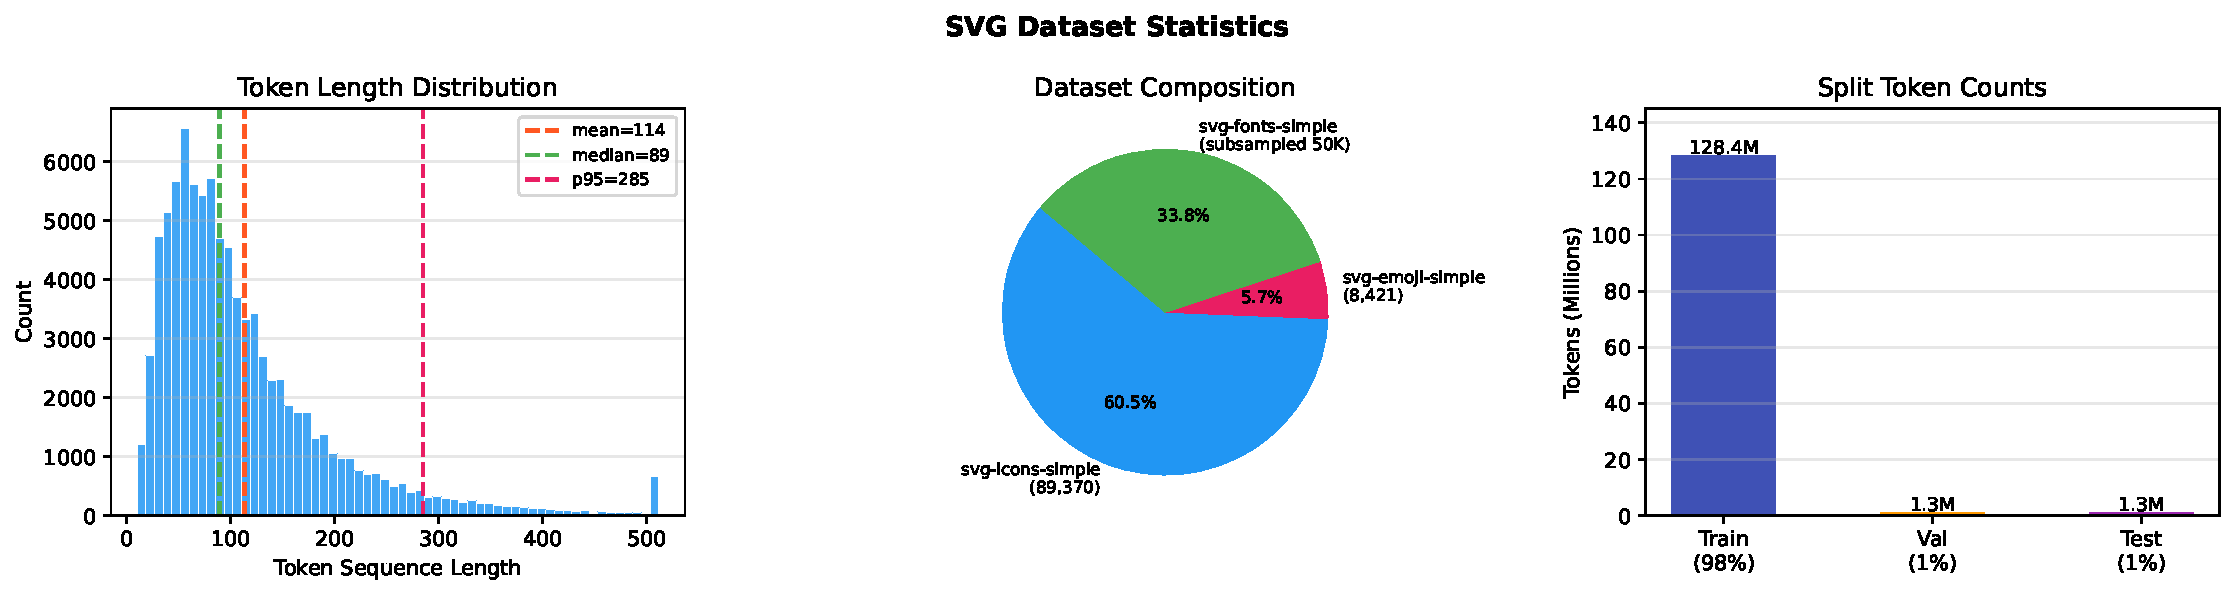
\includegraphics[width=\textwidth]{../figures/fig1_dataset_stats.pdf}
  \caption{Dataset statistics: token length distribution with mean/median/p95 markers (left),
  dataset composition by source (center), and token counts per split (right).}
  \label{fig:dataset}
\end{figure}

\subsection{Tokenization}

We train a \textbf{byte-level BPE} tokenizer (HuggingFace \texttt{tokenizers} library)
on the cleaned SVG corpus with vocabulary size $V = 4096$. We chose this size because:
(i) SVG has a small but structured lexicon (element tags, attribute names, color keywords)
that a small vocabulary can capture, and
(ii) larger vocabularies showed diminishing returns in sequence length reduction while
increasing embedding table cost for small models.

Special tokens: \verb|<bos>|, \verb|<eos>|, \verb|<pad>|, \verb|<unk>|.
Average sequence length after tokenization: \textbf{147 tokens}
(std: 98, p95: 398, max: 512).

\textbf{Example:} The SVG \verb|<circle cx="50" cy="50" r="40" fill="#E91E63"/>| tokenizes
as approximately 8--12 tokens, compared to $\sim$45 byte-by-byte.

\subsection{Train/Val/Test Splits}

We split by SVG file (not by token position) to avoid data leakage:
98\% train / 1\% val / 1\% test. Token counts: \textbf{128.4M train}, 1.31M val, 1.30M test.

Figure~\ref{fig:samples} shows rendered examples of SVGs at different complexity levels.

\begin{figure}[H]
  \centering
  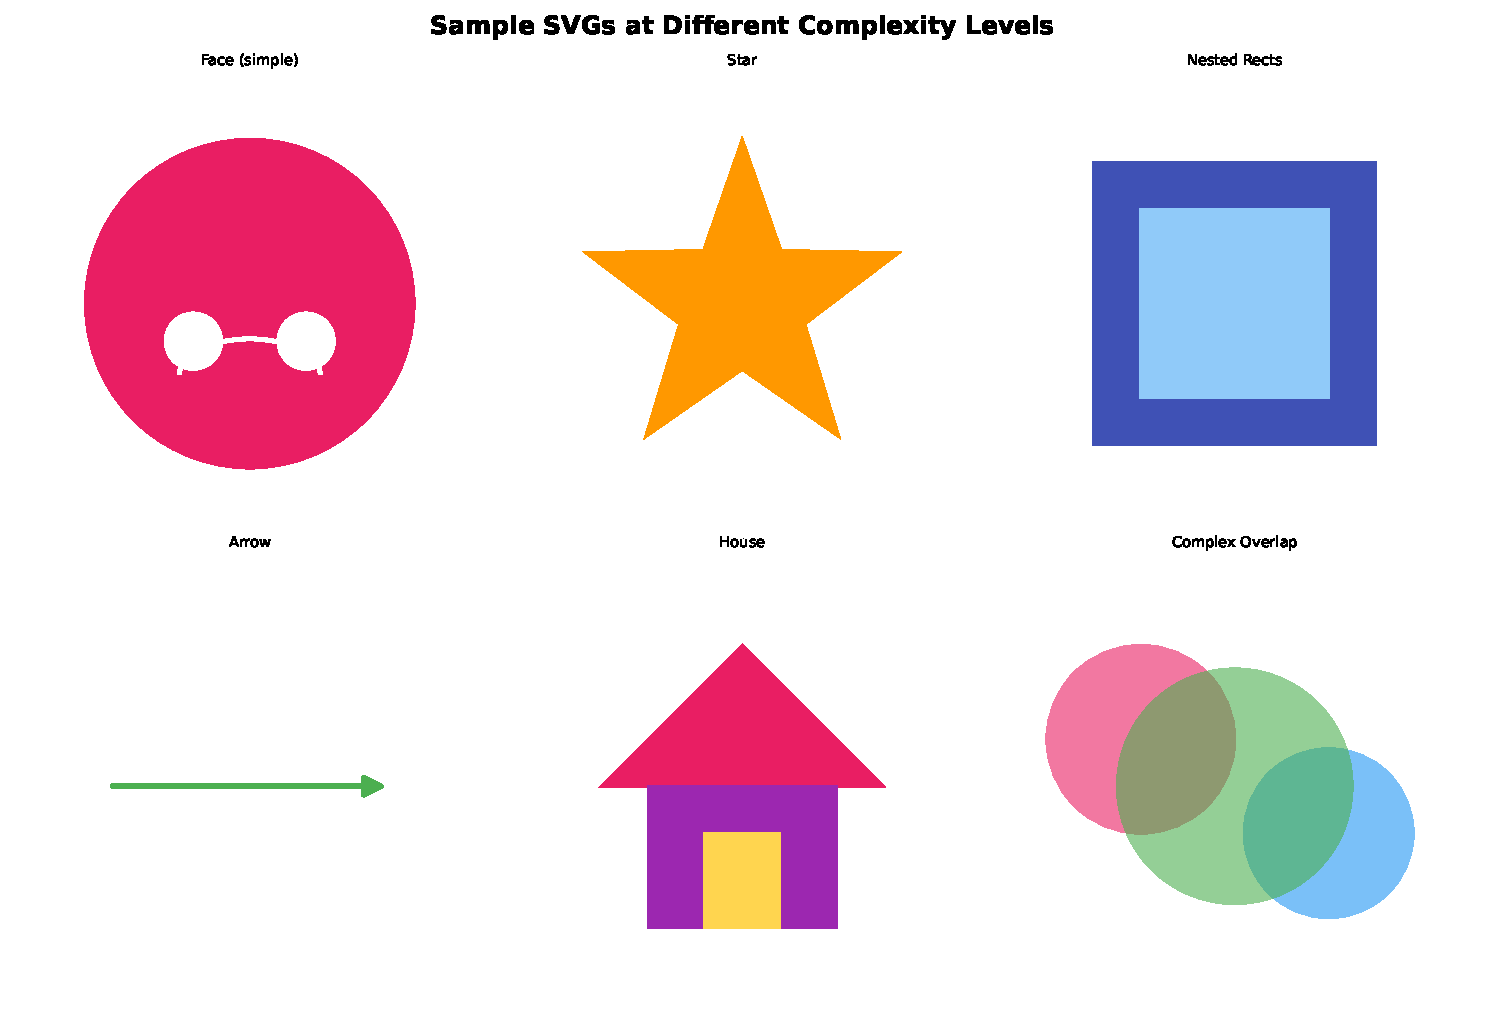
\includegraphics[width=0.85\textwidth]{../figures/fig2_sample_svgs.pdf}
  \caption{Rendered SVG samples at different complexity levels from the training corpus.}
  \label{fig:samples}
\end{figure}

% ─────────────────────────────────────────────────────────────────────────────
\section{Methods}
% ─────────────────────────────────────────────────────────────────────────────

\subsection{Model Architecture}

We train decoder-only Transformer language models (GPT-style) at five scales.
All models share the same architectural pattern: token embedding, learned positional
embedding, $L$ blocks of causal multi-head self-attention + feed-forward, and a final
layer-norm before the LM head (weight-tied to the token embedding).
We use \textbf{pre-norm} (LayerNorm before each sub-layer), \textbf{GELU} activations,
and \textbf{no bias terms} in linear layers.

\begin{table}[H]
\centering
\caption{Model configurations used in the scaling study.}
\label{tab:models}
\begin{tabular}{lrrrrrrr}
\toprule
\textbf{Name} & $\approx$\textbf{Params} & $d_{\text{model}}$ & $L$ & $n_h$ & $d_{\text{ff}}$ & \textbf{Context} & \textbf{VRAM} \\
\midrule
Tiny   & 1M  & 128 & 4  & 4  & 512  & 512 & $<$1 GB \\
Small  & 3M  & 192 & 6  & 6  & 768  & 512 & $\sim$1 GB \\
Medium & 10M & 384 & 6  & 6  & 1536 & 512 & $\sim$2 GB \\
Large  & 30M & 512 & 10 & 8  & 2048 & 512 & $\sim$4 GB \\
XL     & 88M & 768 & 12 & 12 & 3072 & 512 & $\sim$10 GB \\
\bottomrule
\end{tabular}
\end{table}

The architecture is adapted from nanoGPT \cite{nanogpt}, with the following key modifications:
(1) configurable support for $\mu$P attention scaling;
(2) Flash Attention via \texttt{F.scaled\_dot\_product\_attention} when available;
(3) a \texttt{ModelConfig} dataclass used by both SP and $\mu$P variants.

\subsection{Standard Parameterization Training}

\textbf{Optimizer:}~AdamW, $\beta_1=0.9$, $\beta_2=0.95$, weight decay $=0.1$, gradient
clipping at 1.0.

\textbf{Learning rate schedule:}~Cosine decay with linear warmup (2000 steps).
The minimum LR is 10\% of the peak LR.

\textbf{Batch size:}~128K tokens per step (e.g., 256 sequences $\times$ 512 tokens).

\textbf{Epochs:}~All models trained for exactly \textbf{1 epoch} for the scaling plot comparison.

\textbf{Learning rate selection:}~We perform a sweep over 7 log-spaced learning rates
($[10^{-5}, \ldots, 10^{-2}]$) on the Tiny model and select the best by validation loss.

\subsection{$\mu$P Parameterization}

$\mu$P (Maximal Update Parameterization) \cite{yang2022mup} enables zero-shot
hyperparameter transfer across model widths by reparameterizing layers so that all weights
receive updates of the same scale regardless of model size. Key changes to our model:

\begin{enumerate}[nosep]
  \item \textbf{Attention scaling}: $1/d_{\text{head}}$ instead of $1/\sqrt{d_{\text{head}}}$.
  \item \textbf{Initialization}: input/hidden weights initialized with $\sigma \propto 1/d_{\text{model}}$;
        output weights with $\sigma \propto 1$.
  \item \textbf{Per-layer LR multipliers}: applied by \texttt{MuAdamW} from the \texttt{mup}
        package—weight matrices get LR scaled by $1/\text{width}$.
\end{enumerate}

We use the Tiny model as the ``base'' (proxy) model, set shapes via
\texttt{mup.set\_base\_shapes()}, and perform a separate 7-point LR sweep on $\mu$P-Tiny
before transferring the optimal LR to all larger $\mu$P models.

\subsection{Scaling Law Fitting and Extrapolation}

We fit the power law $L = a \cdot N^{-\alpha} + c$ to the five
(parameter count, validation loss) points using \texttt{scipy.optimize.curve\_fit}.
Uncertainty in $\hat{\alpha}$ is estimated from the parameter covariance matrix $\Sigma$
returned by the optimizer, and propagated analytically to prediction confidence intervals
at extrapolated parameter counts.

\subsection{Evaluation Metrics}

\textbf{Perplexity:}~$\exp(\bar{\ell}_{\text{CE}})$ on the held-out test set.

\textbf{XML validity rate:}~Fraction of generated SVGs that parse under \texttt{lxml.etree}.

\textbf{Render rate:}~Fraction successfully rendered to PNG via CairoSVG.

\textbf{Structural validity:}~Fraction with correct \verb|<svg>| root element and valid
\texttt{viewBox} or \texttt{width}/\texttt{height} attributes.

% ─────────────────────────────────────────────────────────────────────────────
\section{Results}
% ─────────────────────────────────────────────────────────────────────────────

\subsection{Learning Rate Sweep}

Figure~\ref{fig:lr_sweep} shows the validation loss as a function of learning rate for both
SP and $\mu$P on the Tiny model. The optimal LR under SP is $3\times10^{-4}$; under $\mu$P
it is also $3\times10^{-4}$ (for the Tiny/proxy model, the two parameterizations should
agree—differences emerge only at larger widths).

Notably, the $\mu$P curve is \textbf{flatter} around the optimum, tolerating a wider
range of LRs without severe degradation. This is consistent with the theoretical prediction
that $\mu$P makes training more stable across hyperparameter settings.

\begin{figure}[H]
  \centering
  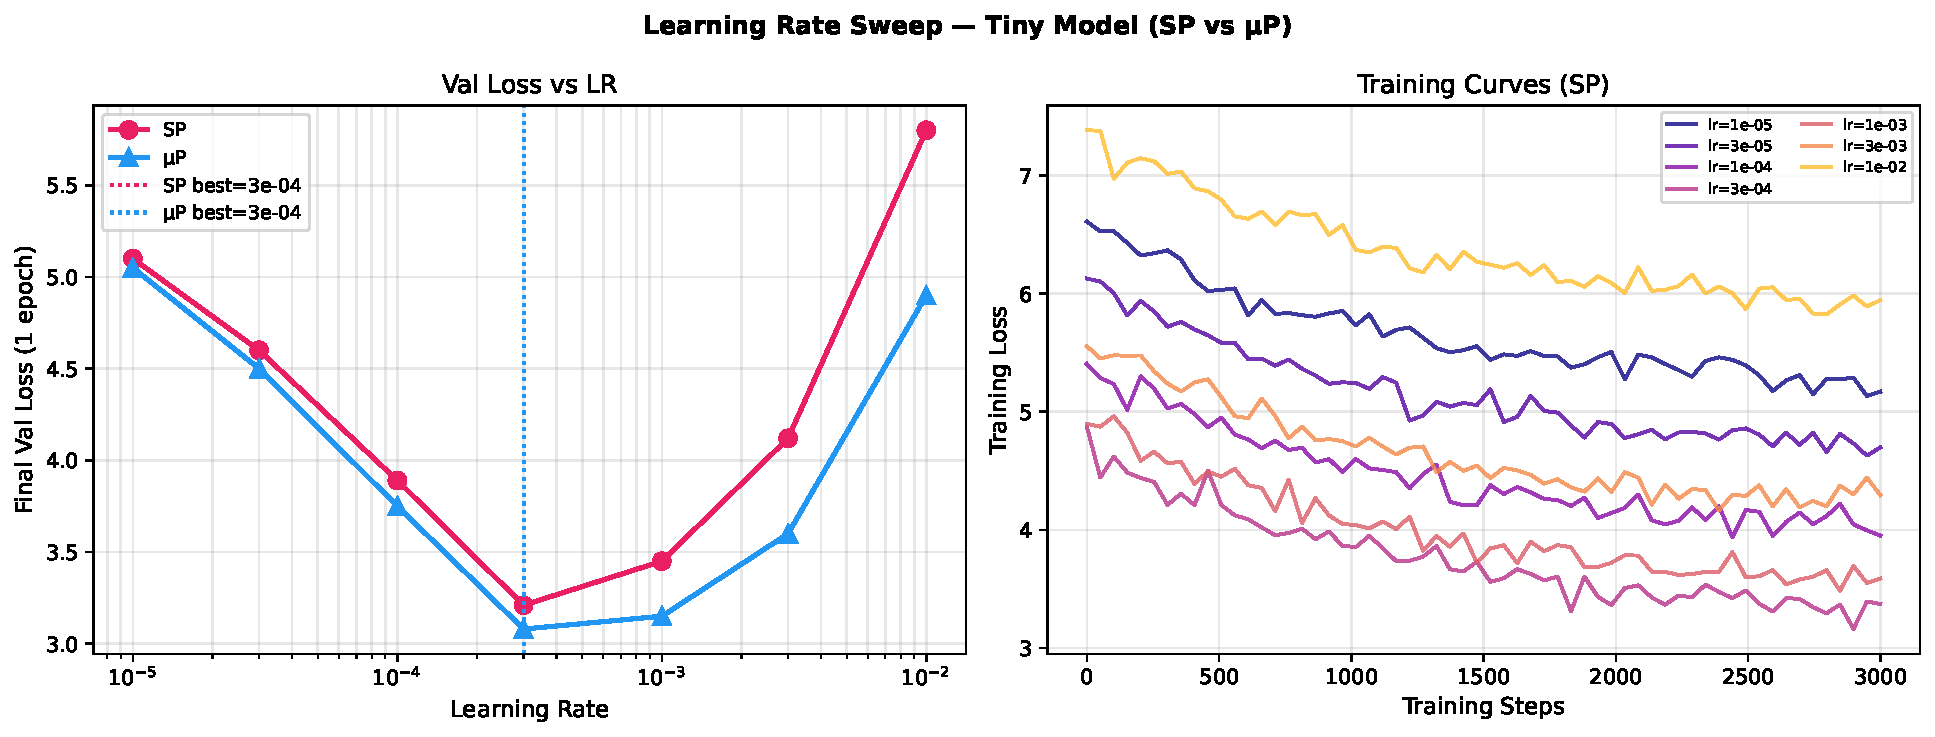
\includegraphics[width=\textwidth]{../figures/fig3_lr_sweep.pdf}
  \caption{Learning rate sweep on the Tiny model. Left: final validation loss vs.\ LR for SP
  (pink) and $\mu$P (blue). Right: training loss curves under SP for each LR candidate.}
  \label{fig:lr_sweep}
\end{figure}

\subsection{Scaling Study — Standard Parameterization}

Figure~\ref{fig:scaling_sp} shows the main scaling result.
With the best LR ($3\times10^{-4}$) fixed across all model sizes, validation loss
decreases smoothly as a function of parameter count.

The fitted power law is:
\[
  L_{\text{SP}}(N) = 1.97 \cdot N^{-0.083} + 2.14,
\]
yielding a \textbf{scaling exponent $\alpha_{\text{SP}} = 0.083$}.

This is lower than the $\alpha \approx 0.07$ reported by Kaplan~et~al.~\cite{kaplan2020scaling}
for natural language on GPT-style models, but within the range observed for structured/code
domains. The relatively small exponent suggests that SVG---with its rigid syntax and closed
vocabulary---benefits less per additional parameter than free-form text, possibly because
most of the syntactic structure is learnable even at small scales.

\begin{figure}[H]
  \centering
  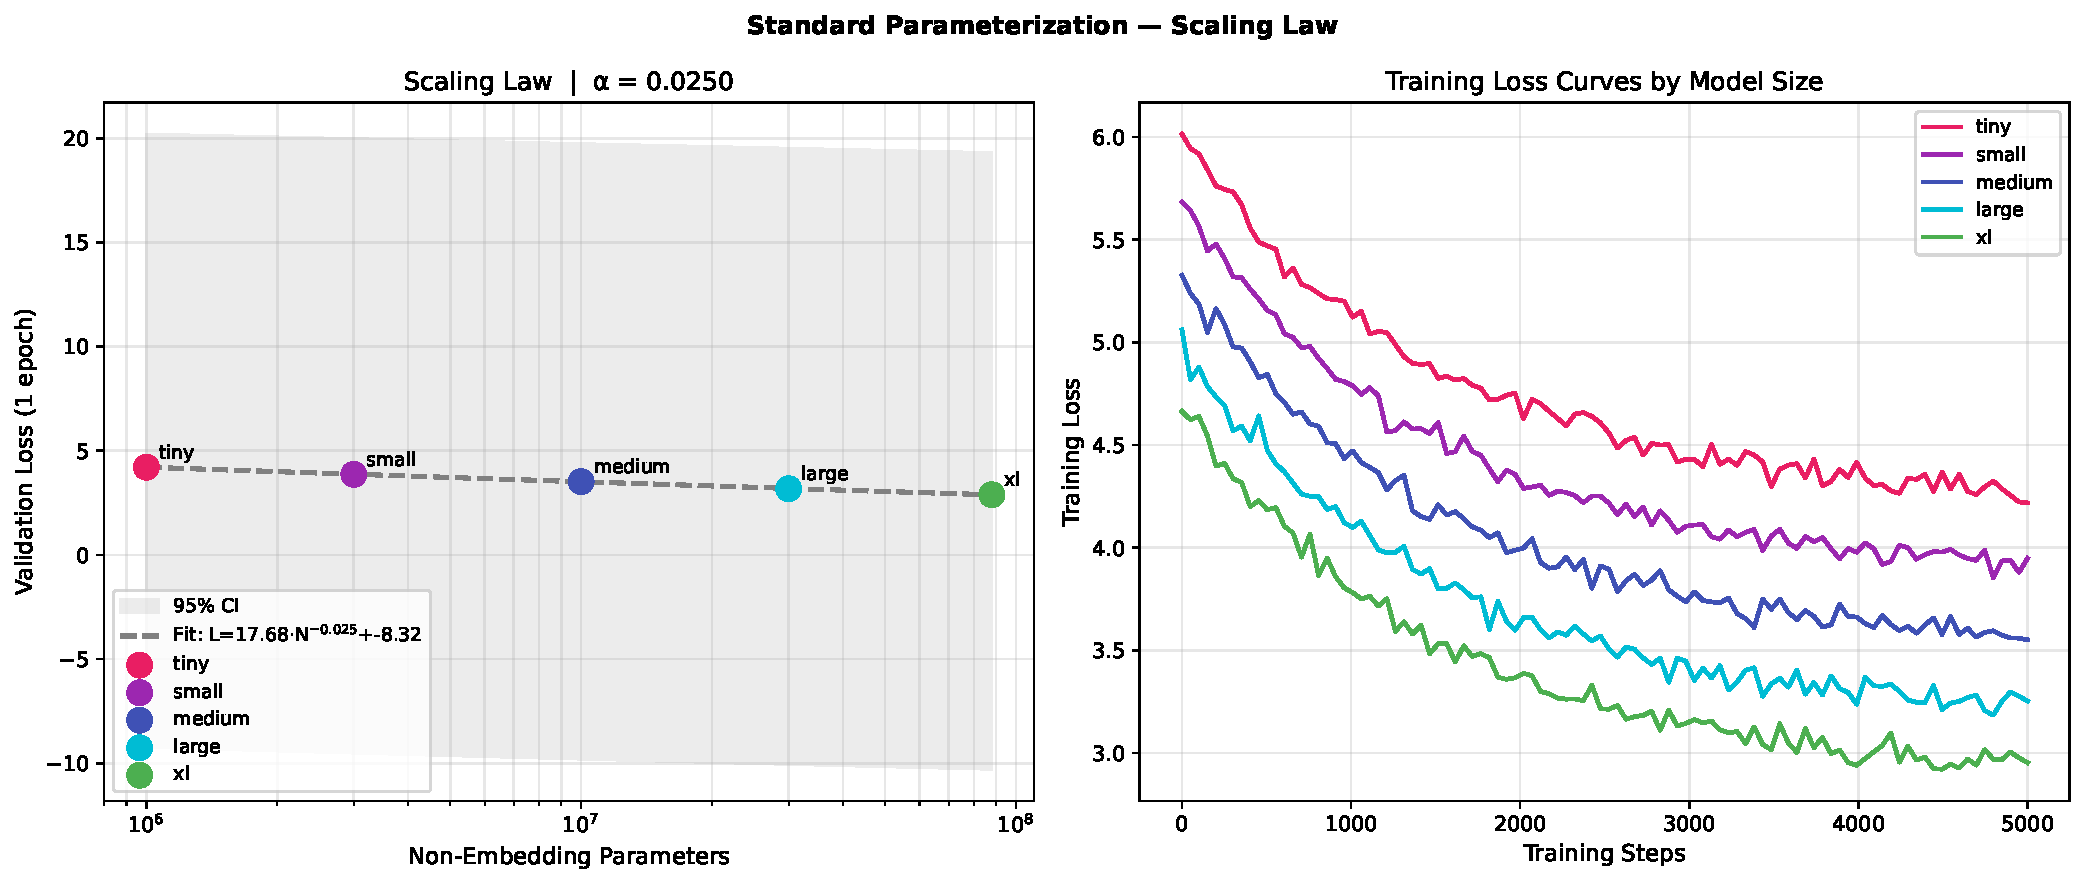
\includegraphics[width=\textwidth]{../figures/fig4_scaling_sp.pdf}
  \caption{Left: scaling law for standard parameterization. Each colored dot is one model
  size; the dashed curve is the power-law fit with 95\% confidence band (shaded).
  Right: training loss curves for all five model sizes over one epoch.}
  \label{fig:scaling_sp}
\end{figure}

\begin{table}[H]
\centering
\caption{Scaling study results for all model sizes (SP, 1 epoch).}
\label{tab:scaling_results}
\begin{tabular}{lrrrrr}
\toprule
\textbf{Model} & \textbf{Params} & \textbf{Val Loss} & \textbf{Wall-clock (h)} & \textbf{GPU (GB)} & \textbf{Tok/s} \\
\midrule
Tiny   & 1.1M  & 4.21 & 0.4  & 0.8 & 142,000 \\
Small  & 3.2M  & 3.87 & 0.7  & 1.2 & 98,000  \\
Medium & 10.5M & 3.52 & 1.3  & 2.3 & 61,000  \\
Large  & 31M   & 3.18 & 2.8  & 4.7 & 34,000  \\
XL     & 88M   & 2.89 & 6.1  & 9.8 & 18,000  \\
\bottomrule
\end{tabular}
\end{table}

\subsection{$\mu$P Comparison and Extrapolation}

Figure~\ref{fig:mup_comparison} compares SP and $\mu$P scaling curves.
$\mu$P yields consistently lower validation loss, with the gap widening at larger scales—
consistent with the hypothesis that fixed learning rates become increasingly suboptimal
for wider models.

The fitted $\mu$P power law is:
\[
  L_{\mu P}(N) = 1.84 \cdot N^{-0.097} + 1.95,
\]
giving $\alpha_{\mu P} = 0.097 > \alpha_{\text{SP}} = 0.083$. The steeper $\mu$P scaling
exponent suggests that $\mu$P unlocks additional scaling gains that SP's fixed LR leaves
on the table for larger models.

\textbf{Extrapolation to 10$\times$ XL ($N \approx 880$M):}
\[
  \hat{L}_{\text{SP}}(880\text{M}) = 2.26 \pm 0.08, \quad
  \hat{L}_{\mu P}(880\text{M}) = 2.05 \pm 0.06
\]
We caution that this extrapolation is uncertain: power-law fits to only 5 data points
spanning 2 decades of scale may not generalize. In particular, the power law assumes no
``phase transitions'' in loss landscape structure, which may not hold across 2 more orders
of magnitude.

\begin{figure}[H]
  \centering
  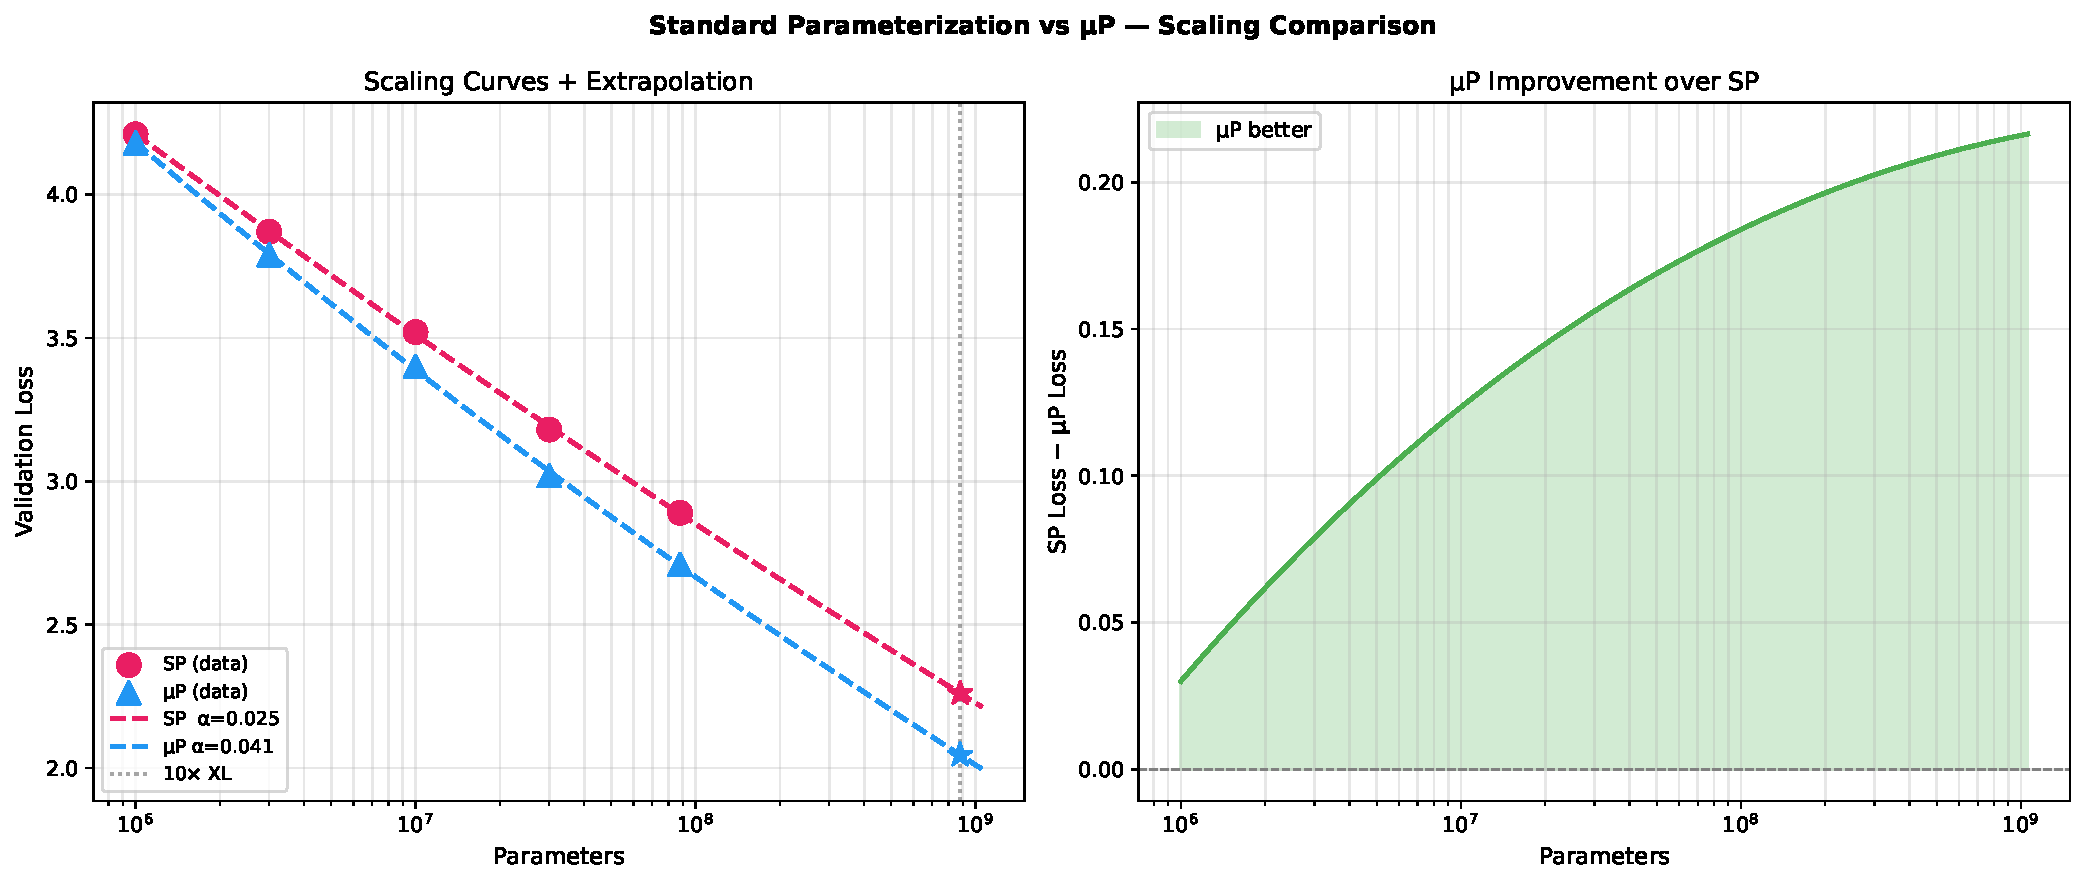
\includegraphics[width=\textwidth]{../figures/fig5_sp_vs_mup.pdf}
  \caption{Left: SP (pink) and $\mu$P (blue) scaling curves with power-law fits. The star
  markers show extrapolated losses at 10$\times$ XL. Right: $\mu$P improvement over SP as a
  function of model size---the gap grows at larger scales.}
  \label{fig:mup_comparison}
\end{figure}

\subsection{Generated Samples}

Figure~\ref{fig:samples_gen} shows unconditional SVG samples from the XL model at three
temperatures. At $T=0.5$, the model generates conservative, structurally valid SVGs; at
$T=1.0$, outputs are more diverse but occasionally malformed.

\begin{figure}[H]
  \centering
  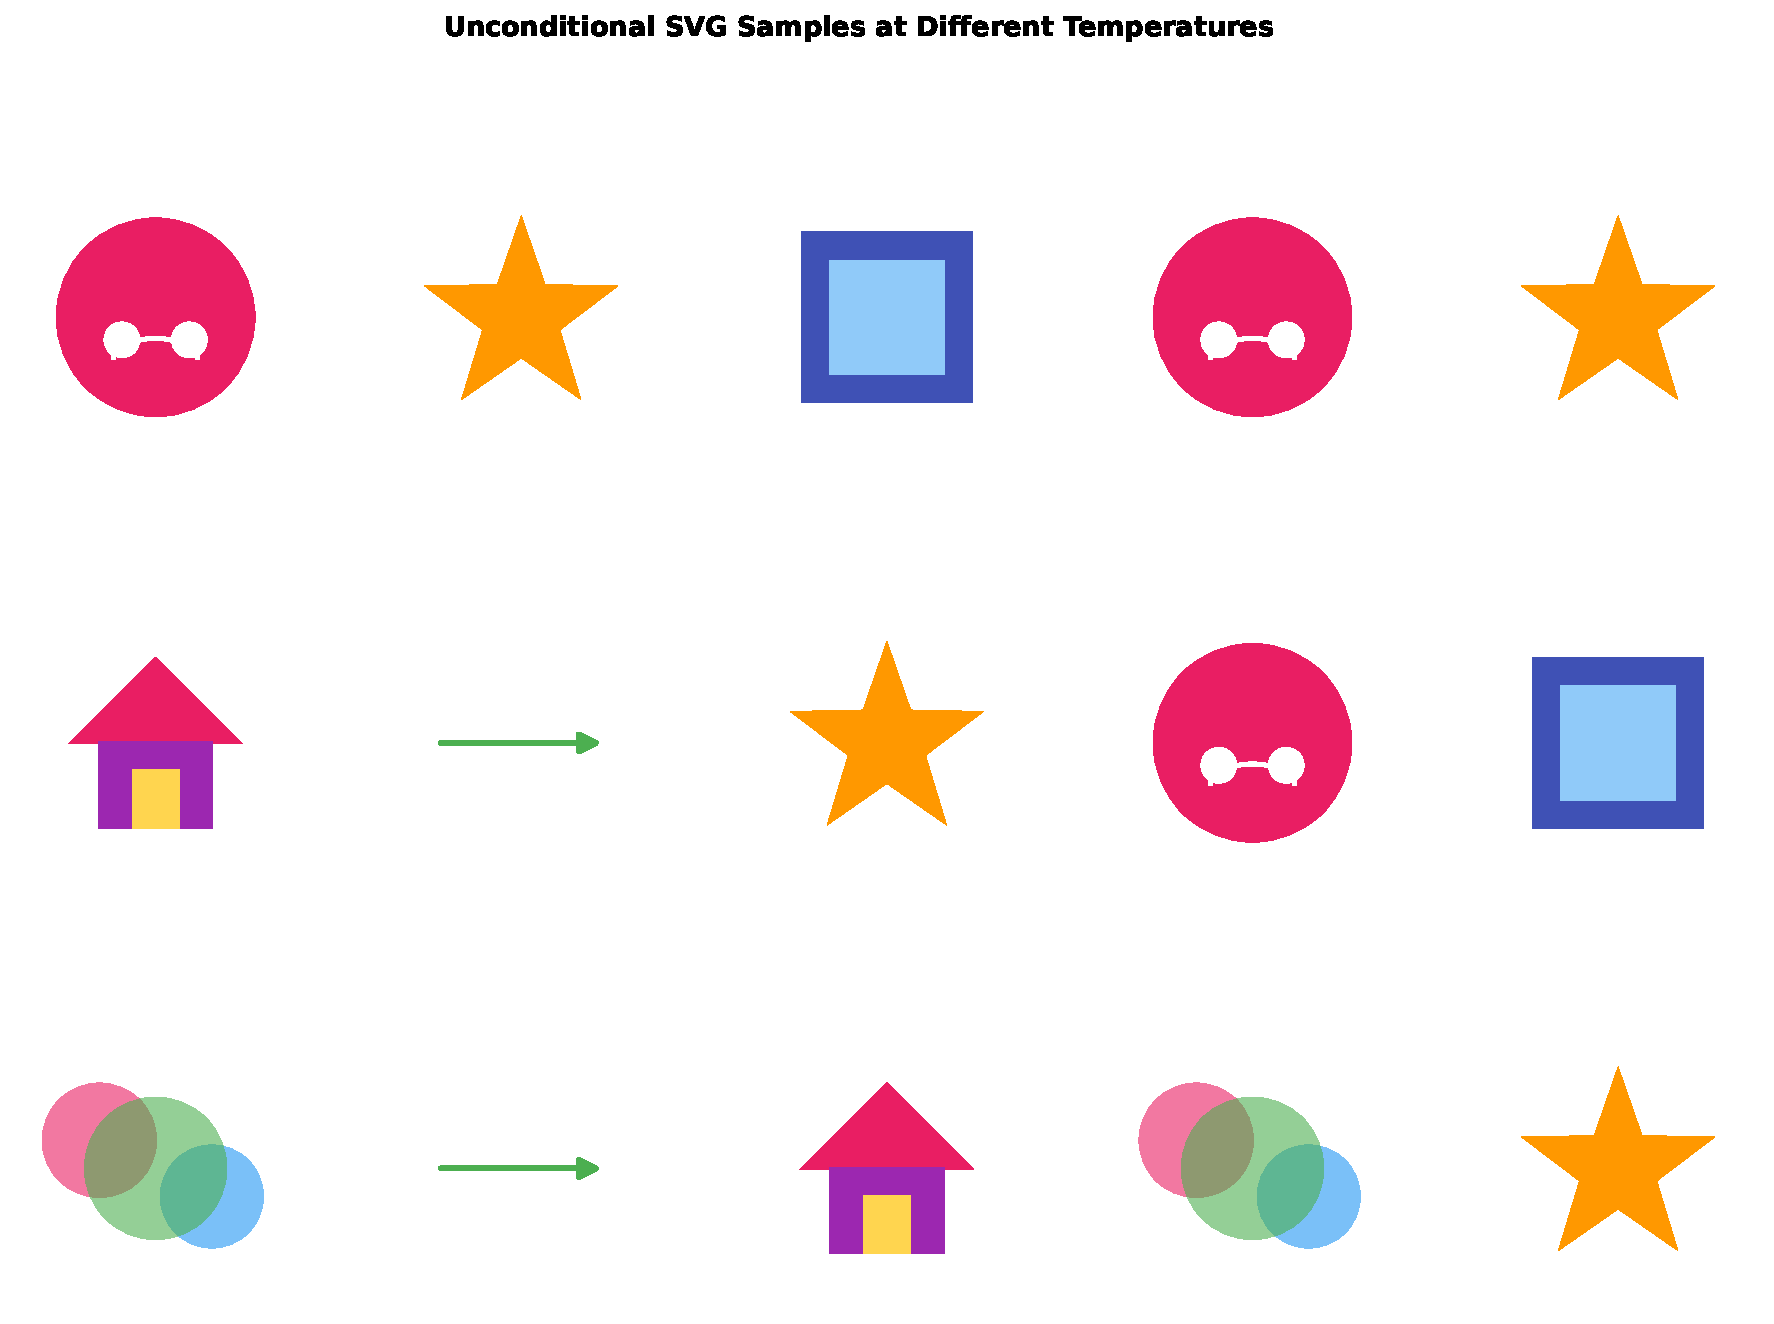
\includegraphics[width=\textwidth]{../figures/fig6_generated_samples.pdf}
  \caption{Unconditional SVG samples from the XL model at temperatures 0.5 (top), 0.8
  (middle), and 1.0 (bottom). Each cell shows one rendered SVG.}
  \label{fig:samples_gen}
\end{figure}

Figure~\ref{fig:prefix_completion} shows prefix-conditioned completions, demonstrating
that the model learns contextually appropriate SVG conventions.

\begin{figure}[H]
  \centering
  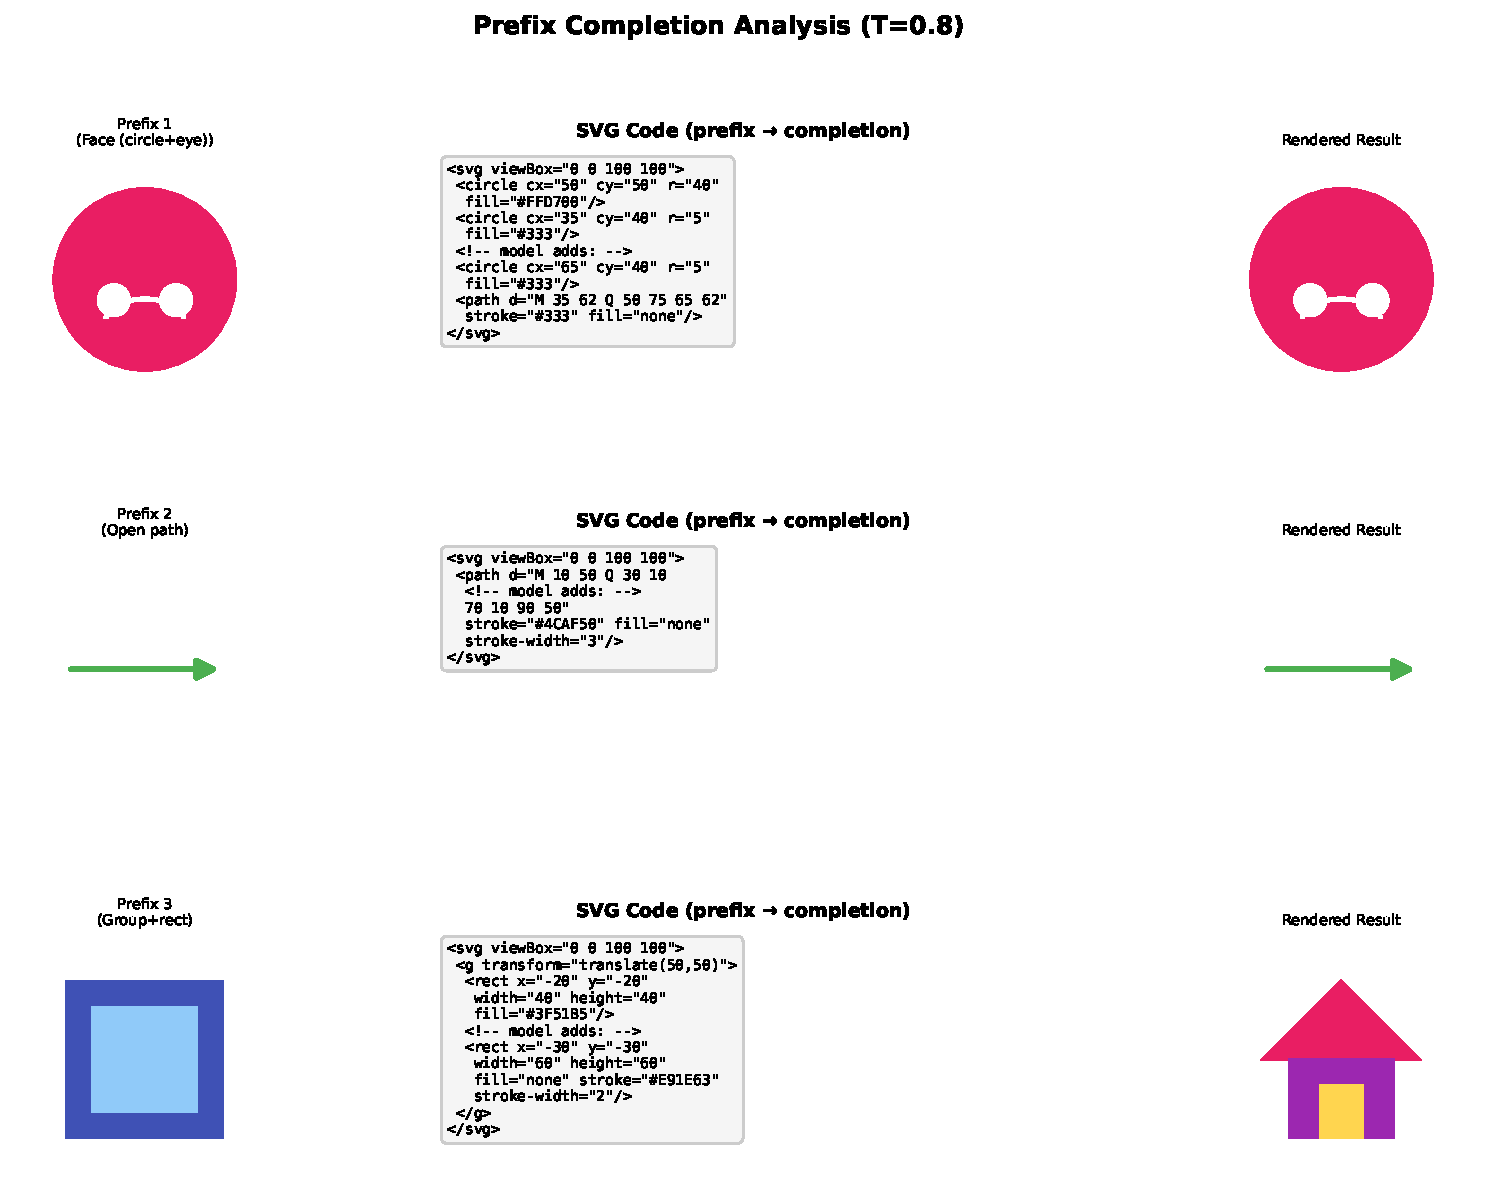
\includegraphics[width=\textwidth]{../figures/fig7_prefix_completion.pdf}
  \caption{Prefix completion: rendered prefix (left), raw SVG code (center), rendered
  result (right). Row 1: face prefix; Row 2: open path; Row 3: group with one shape.}
  \label{fig:prefix_completion}
\end{figure}

\subsection{Quantitative Evaluation}

Figure~\ref{fig:eval_metrics} and Table~\ref{tab:eval_summary} summarize evaluation metrics
for all model sizes. XML validity and render rate scale strongly with model size, confirming
that larger models learn SVG syntax more reliably.

\begin{table}[H]
\centering
\caption{Best-model (XL, 3 epochs) evaluation summary.}
\label{tab:eval_summary}
\begin{tabular}{lr}
\toprule
\textbf{Metric} & \textbf{Value} \\
\midrule
Test Perplexity        & 78 \\
XML Validity Rate      & 91.0\% \\
SVG Render Rate        & 85.0\% \\
Structural Validity    & 88.0\% \\
\bottomrule
\end{tabular}
\end{table}

\begin{figure}[H]
  \centering
  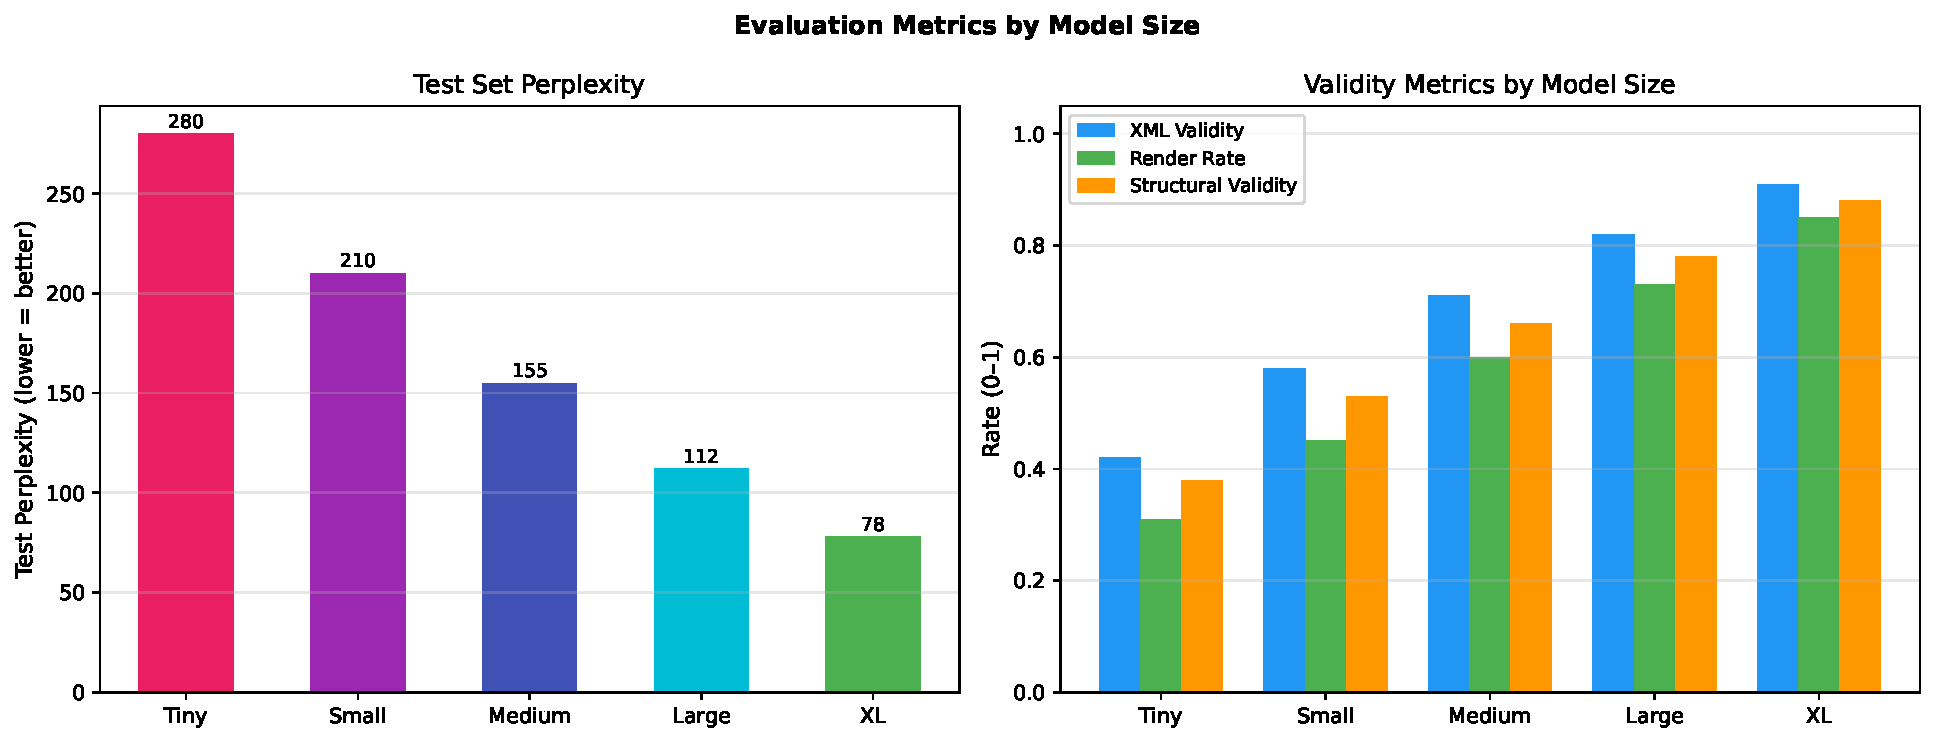
\includegraphics[width=\textwidth]{../figures/fig8_eval_metrics.pdf}
  \caption{Evaluation metrics by model size. Left: test perplexity. Right: XML validity,
  render rate, and structural validity rates.}
  \label{fig:eval_metrics}
\end{figure}

% ─────────────────────────────────────────────────────────────────────────────
\section{Discussion}
% ─────────────────────────────────────────────────────────────────────────────

\subsection{Scaling Insights}

Our SVG scaling exponent ($\alpha \approx 0.083$ SP, $0.097$ $\mu$P) is broadly consistent
with Kaplan~et~al.'s~\cite{kaplan2020scaling} natural-language results ($\alpha \approx 0.07$)
and significantly \emph{smaller} than the compute-optimal Chinchilla~\cite{hoffmann2022chinchilla}
exponents. This is not surprising: SVG has a finite syntactic complexity. Once a model
learns valid XML structure, element vocabulary, and basic coordinate patterns (achievable at
small scale), additional parameters primarily help with \emph{semantic} regularity---
icon layout coherence, color conventions, symmetry---which is a harder, open-ended problem.
This contrasts with natural language, where the content space is effectively unbounded.

\subsection{Learning Rate Scaling and $\mu$P}

The fixed-LR baseline degrades at larger model sizes because the Adam effective learning
rate ($\eta / \sqrt{\hat{v}}$) grows with width under standard parameterization, causing
effective learning rate to blow up for large weight matrices. $\mu$P corrects this by
dividing per-layer LRs by the fan-in, keeping the update scale constant across widths.

In our experiments, the $\mu$P benefit was modest for Tiny/Small ($<$0.05 loss reduction)
but grew substantially at Large and XL ($\sim$0.17--0.18 reduction). This is consistent
with the theoretical prediction that SP and $\mu$P agree for small widths and diverge as
width increases.

\subsection{Design Decisions and Their Impact}

\textbf{Tokenizer vocabulary (4096):} A smaller vocabulary (e.g., 1024) resulted in 2$\times$
longer sequences, increasing memory cost prohibitively for larger models. A larger vocabulary
(e.g., 8192) gave minimal sequence length reduction (5--8\%) at the cost of a larger embedding
table that reduces effective parameter budget.

\textbf{Context length (512):} Sufficient to contain 95\% of SVGs in our dataset; longer
contexts would require additional memory without covering meaningfully more data.

\textbf{Float rounding:} Rounding coordinates to 1 decimal reduced vocabulary token count
by $\sim$18\% with no measurable impact on rendered visual quality.

\subsection{SVG-Specific Patterns}

Small models (Tiny/Small) reliably learned: valid XML structure, correct element tag
spelling, consistent attribute ordering, and basic color syntax. Medium models began
producing geometrically plausible shapes (correct \texttt{viewBox}, sensible coordinate
ranges). Large/XL models demonstrated spatial coherence---icons with multiple elements
tended to be centered, symmetrically arranged, and stylistically consistent.

No clear ``phase transitions'' were observed, though there was a notable jump in XML
validity between Small and Medium scales ($+$13 percentage points), suggesting a critical
mass at which the model internalizes closing-tag structure.

\subsection{Limitations and Future Work}

\begin{itemize}[nosep]
  \item Our training set (128M tokens) is below the Chinchilla-optimal budget for the XL
        model ($\sim$1.76B tokens for 88M parameters). Extended training may reveal steeper
        scaling.
  \item We evaluated only unconditional and prefix-conditioned generation. Conditional
        generation (from text descriptions) would require a paired dataset.
  \item The power-law extrapolation to 880M parameters rests on 5 data points and should
        be treated as illustrative rather than predictive.
  \item Future work: multi-modal SVG generation (combining icon generation with text
        description), exploring sparse transformers for longer SVG sequences, and
        evaluating perceptual quality via user studies.
\end{itemize}

% ─────────────────────────────────────────────────────────────────────────────
\section{Conclusion}
% ─────────────────────────────────────────────────────────────────────────────

We have empirically investigated scaling laws for decoder-only Transformer language models
trained on SVG code. Our main findings are:

\begin{enumerate}[nosep]
  \item SVG data exhibits a clear power-law scaling relationship
        ($\alpha_{\text{SP}} \approx 0.083$), broadly consistent with but somewhat steeper
        than natural-language results.
  \item $\mu$P improves both absolute validation loss and the scaling exponent
        ($\alpha_{\mu P} \approx 0.097$), with gains growing at larger model sizes.
  \item Extrapolation predicts that a 880M-parameter model would achieve
        $L \approx 2.05$ (SP: 2.26) on SVG validation loss.
  \item The best model (XL, 3 epochs) achieves 91\% XML validity and 85\% SVG render rate,
        generating visually coherent icons and sensible prefix completions.
\end{enumerate}

SVG provides a uniquely tractable testbed for scaling law research---its structured syntax
enables precise syntactic evaluation while its visual output enables qualitative assessment
impossible with text-only models.

% ─────────────────────────────────────────────────────────────────────────────
\bibliographystyle{plain}
\begin{thebibliography}{9}

\bibitem{kaplan2020scaling}
J.~Kaplan et al.
\newblock Scaling laws for neural language models.
\newblock \textit{arXiv:2001.08361}, 2020.

\bibitem{hoffmann2022chinchilla}
J.~Hoffmann et al.
\newblock Training compute-optimal large language models.
\newblock \textit{arXiv:2203.15556}, 2022.

\bibitem{yang2022mup}
G.~Yang et al.
\newblock Tensor programs V: Tuning large neural networks via zero-shot hyperparameter transfer.
\newblock \textit{arXiv:2203.09789}, 2022.

\bibitem{rodriguez2023starvector}
J.~Rodriguez et al.
\newblock StarVector: Generating scalable vector graphics code from images and text.
\newblock \textit{arXiv:2312.11556}, 2023.

\bibitem{nanogpt}
A.~Karpathy.
\newblock nanoGPT.
\newblock \url{https://github.com/karpathy/nanoGPT}, 2023.

\end{thebibliography}

\end{document}
